\documentclass[conference]{IEEEtran}
\usepackage{cite}
\usepackage{amsmath,amssymb,amsfonts}
\usepackage{algorithmic}
\usepackage{graphicx}
\usepackage{textcomp}
\usepackage{xcolor}
\usepackage{tabularx}
\usepackage{hyperref}
\def\BibTeX{{\rm B\kern-.05em{\sc i\kern-.025em b}\kern-.08em
    T\kern-.1667em\lower.7ex\hbox{E}\kern-.125emX}}
\begin{document}

\title{ARGUS: Analytical Reasoning and Grounded Understanding System}

\author{
\IEEEauthorblockN{
Willow Dennison\IEEEauthorrefmark{1},
Luna Smith\IEEEauthorrefmark{2},
Ajit Chavan, Ph.D.\IEEEauthorrefmark{3},
and Ann Cannon, Ph.D.\IEEEauthorrefmark{4}
}

\IEEEauthorblockA{
\textit{\IEEEauthorrefmark{1}Computer Science, Data Science}
\textit{\IEEEauthorrefmark{2}Computer Science} \\
\textit{\IEEEauthorrefmark{3}Associate Professor, Computer Science}
\textit{\IEEEauthorrefmark{4}Watson M. Davis Professor of Mathematics and Statistics}\\
\textit{Cornell College, Mount Vernon, Iowa, United States}\\
Emails: wdennison26@cornellcollege.edu,
msmith26@cornellcollege.edu,\\
achavan@cornellcollege.edu,
acannon@cornellcollege.edu
}
}

\maketitle

\begin{abstract}
% Fake news! It is bad.
Enter ARGUS: an application that uses LLMs to analyze the accuracy and completeness of web articles. With the rise of AI generated content online, reliable fact checking is more important than ever; we built an application to use LLMs to automate the process of debunking articles to counter this rise of misinformation. While quantifying truth is all but impossible, we can cross reference an article with other articles on the same topic or other background information to form a close approximation. The articles on the same topic can be used to compare the completeness of the information reported, and the background information can be used to fact check the claims in the article itself. Those two measures can be combined for a largely accurate measure of the ``truthfulness" of the article -- if the reporting is factually accurate and the article includes all the relevant information, it's reasonable to consider it truthful. In addition to the quality of fact check output, the development process took into account the efficiency of the overall application, measured by the number of LLM prompts and overall processing time per article. Running on consumer hardware, ARGUS delivers fact checks in 10-30 minutes, competitive with state-of-the-art tools, while remaining fully open source and locally deployable.
\end{abstract}
% find SOMEWHERE to elaborate on how we're doing the accuracy and completeness scores. yeah its mostly vibes but we gotta say "yeah its mostly vibes but there isnt really another choice. doing it multiple times should help with accuracy but well need to refine a lot in the prompt engineering stage.

\begin{IEEEkeywords} %lol. lmao.
LLM - Large Language Model
\end{IEEEkeywords}

\section{Introduction}
Between the rise of social media and of AI generated content online, plenty has been said about the increased dangers of misinformation in the modern day, and about how we can detect and counter it. ``Fake news" has been a common buzzword and political rallying cry since at least 2016, but the consequences are measurable. There is evidence that misinformation influenced the outcome of the 2016 US presidential election; only 77\% of former Barack Obama supporters voted for Hillary Clinton in 2016, and analysis shows that a statistically significant number of them abandoned support over misinformation, enough to lose her the election\cite{2016ElectionStats}. Exposure to COVID-19 vaccine misinformation has been shown to increase vaccine hesitancy, which feasibly could have prolonged the pandemic\cite{Loomba2021}. The increasing prevalence of AI generated misinformation -- both intentional disinformation and hallucinations -- presents new challenges for traditional means of misinformation detection, requiring new adaptations for our existing detection tools\cite{Zhou2023}.

%paragraph 2: existing applications for detecting fake news, llm based deep research / non llm based solutions
Existing solutions for misinformation detection have their advantages, there was a gap for us to fill. Ground News is a site that aggregates news articles on specific topics to compare how different sources report on it, but the articles have to be selected manually, they only display certain popular topics, and most of their features require a paid subscription\cite{groundNews}. Snopes is a veteran fact checking site, both for specific claims and for full articles, but their system is entirely manually written and requires a staff to actively prove or disprove the claims\cite{Snopes}. Automated solutions, usually LLM-based, exist as well, but they too have disadvantages. The chatbot LLM Grok\cite{Grok4}, integrated into X (formerly Twitter), has become very popular for fact checking claims\cite{esteban_ponce_de_leon_grok_2025}, but it's optimized for witty, entertaining responses rather than the most factually correct answers\cite{xai_xai_announcing_2023}. The opposite end of the spectrum is ChatGPT Deep Research\cite{DeepResearch}, a rigorously tested system that outputs full research reports on topics of the user's request, but it's limited to paid users and can take upwards of 30 minutes per report\cite{introducingDR}.

%paragraph 3: what is our solution for fake news: ARGUS
ARGUS bridges the gap between the accessibility and ease of use of Grok and the commitment to factuality of Deep Research. It quickly and efficiently scans through articles provided by the user using open source LLMs -- either hosted locally or on any OpenAI API compatible server -- and searches the web for reliable sources to verify or disprove its claims. It searches for articles on the same topic and uses LLM calls to compare differences and evaluate potential reporting bias. It then combines all that into a summary of what was correct, what was incorrect, reporting bias, and citations for all of its sources within a few minutes. While similar tools for fact checking news articles exist, ARGUS automates the process of fact checking on a scale that could feasibly be run on a home computer in 10-30 minutes, which is competitive with state-of-the-art tools, and is fully open source in the name of accessibility. The project, on top of building a functional and useful open source application, also provided the authors excellent professional experience using LLMs, web scraping, and web application and API development.

\section{Related Work}

\subsection{Ground News}
Ground News is a platform that aggregates news articles on specific topics to highlight differences in reporting across the political spectrum\cite{groundNews}. The platform also features factuality ratings for some articles, but the feature is only available to paid users\cite{groundNewsSubscriptions}. Free tier users are greeted with a homepage full of news topics, with the political distribution of the outlets reporting on it (either left, right, or center). These political bias ratings are determined per reporting source from outside sources that audit media bias (including but not limited to mediabiasfactcheck.com). Paid users gain access to a ``blind spot" feed that analyzes what news sources the user tends to consume and selects topics to show them that they would be unlikely to see otherwise. They also offer factuality ratings for some articles, but these are only available to paying users\cite{groundNews}.

ARGUS follows a similar philosophy, the goal being to cut through media bias and misreporting, but it takes a more narrow, fully automated approach, and is fully accessible for free. Where Ground News focuses on topics, ARGUS focuses on checking the factuality and completeness of individual articles provided by the user. Ground News' factuality ratings are relatively minimal in terms of explanation, where ARGUS writes you a summary of the factuality and bias of the article with cited sources for free. In ARGUS, the LLM evaluates bias ratings based on both the reputation of the source and the specific article at hand, allowing bias ratings to be article specific rather than a blanket score for the source.

\subsection{Grok}
Grok is a chatbot LLM produced by xAI, integrated into X (formerly Twitter), which is often used for fact checking in online arguments\cite{esteban_ponce_de_leon_grok_2025}. Grok's latest version, Grok 4, like most state of the art chatbots, is capable of searching the web for sources to inform its responses, as well as having live access to any and all content on the platform itself. This leads to the interesting situation of a tool that is frequently used for fact checking, but, as a chatbot, it's finetuned for engaging responses rather than the most accurate. It has the ability to cite its sources, and often does, but they will sometimes be left out for brevity,  highlighting the focus on entertainment over factuality\cite{Grok4}. Many sources have criticized the xAI team for their lack of emphasis on guardrails in the training process, allowing users to generate illegal content with relative ease, but these issues also carry over into the factuality of its corrections\cite{MediumGrokGuardrails}.

ARGUS intentionally foregoes the entertainment value to provide the most straightforward and accurate fact checking experience: a user provides an article, they get a report with cited sources on what it does right and wrong. Where the Grok LLM is free to check its sources at its own discretion, ARGUS follows a rigid call structure that will always find sources to back up or disprove all of the major claims in the article. The focus on procedure and requiring sources for every claim helps with providing the most factually robust summaries possible and allowing users to verify anything ARGUS says with ease. 

\subsection{ChatGPT Deep Research}
Deep Research is an AI agent produced by OpenAI based on a specialized version of their o3 model\cite{introducingDR}. It creates ``comprehensive reports with breadth, depth, and precision," compiling information from hundreds of web sources\cite{DeepResearch}. It also includes a ``lightweight" version running on the o4 mini model, which is available more frequently and for cheaper. Only the lightweight model is available to free tier users, and they're limited to 5 queries per month. The mainline Deep Research model is exclusively available to paid users with monthly limits. Performing robust research and citing reliable sources for a complex topic is extremely expensive in terms of computing power, so it's sensible to limit users to this extent, but it necessarily inhibits accessibility. The agent also runs on an extremely high end LLM, which provides the best results but at the cost of huge amounts of processing power and large time costs -- Deep Research requests can take upwards of 30 minutes for a sufficiently complex topic\cite{DeepResearch}.

Deep Research and ARGUS follow similar processes and work on the same ideas: getting the most factually accurate summary by scraping the web and using LLMs to summarize findings. ARGUS plans to take a more narrow approach, specifically tailoring the process to fact checking news articles. This is in part due to practical reasons -- we don't have easy access to high end models or entire data centers to run them -- but our approach is a lot more user friendly and transparent; a 3 paragraph summary with 5-10 sources is much easier to scroll through than a multi page research report. There's also the time factor, Deep Research takes between 5 and 30 minutes to output its report running on state of the art technology. ARGUS, in comparison, can output in under 30 minutes running on a typical gaming PC, and can be sped up drastically when running models on multiple machines with distributed computing (under 15 minutes with our available hardware, but there is theoretically no limit to the improvement).

\subsection{Snopes}
Snopes is one of the most famous fact checking sites, based on taking popular claims and verifying them manually\cite{Snopes}. Having been around since 1994, it has gained a reputation as a reliable source for proving or disproving internet rumors\cite{Snopes}. The biggest difference between Snopes and ARGUS is that every Snopes article is written by a real person. This certainly improves reliability, hallucination becomes a complete non-issue, but it slows down the process. In contrast, ARGUS offers on demand fact checking for any article the user wants.

\section{System Design}
\subsection{Graphical User Interface}
The graphical user interface serves as the primary method for users to fact-check articles. It provides a simple to use interface that can expose a wide variety of information about the analyzed articles. The front end is built using React with Tailwind CSS for styling, which helps to keep the interface clean and responsive while giving us a lot of flexibility in UI design \cite{react, tailwind}.

\subsubsection{Home Page}
The home page provides users with a straightforward entry point to the fact-checking system. Users are able to paste an article URL into a prominent input field and start the analysis with a single click. The page also includes a brief explanation of how the tool works and what users can expect from the analysis. Additionally, the home page displays recent analyses to help users discover relevant or interesting fact-checks.

\subsubsection{Article Analysis Page}
Once an article has been submitted and begins processing, users are directed to the analysis page where the results are summarized and displayed. As the system works, the page automatically fills in sections that the system has finished processing to reduce user downtime. The page is split into several sections that work together to provide a comprehensive fact-check.

The first section is an article summary generated by the LLM, which will contain the input article's main points and primary claims. This gives users a quick overview of what the article asserts, and what our system will then be verifying. For each article, the source, publication date, and a brief summary are shown.

The gathered information is then passed to three separate AI agents -- the accuracy, bias, and completeness evaluation agents. These are instances of LLMs equipped with tools to research their analyses, primarily to search the internet and the existing database for background information. When the agents feel that they have enough information to make their final assessments, they return their outputs: an accuracy score from 0-100 and an explanation, a completeness score from 0-100 and an explanation, and bias scores from 0-100 with explanations for political bias, sensationalism, and emotional language respectively.

\subsubsection{Data Sandbox}
The data sandbox provides an interactive space for users to explore patterns and trends in the articles that have been analyzed by the system. This feature serves both as a research tool and a way to understand broader patterns in news coverage and misinformation across the articles stored in the database. Users are able to visualize data through various interactive charts (using ggplot2) and graphs, filter and drill down into the data, and export their findings for further analysis in other programs \cite{ggplot}. The data sandbox offers both a basic and advanced mode: the basic mode offering a few interactive graphs, and the advanced mode offers a full R console (implemented with WebR) for users to perform their own data analysis \cite{webr}.

\subsubsection{Other Features}
Dedicated mobile support for ARGUS has been implemented, as well as a webhook-based notification system. Future versions may include a browser extension to automatically submit articles, user accounts, or a more robust issue reporting system.

\section{System Architecture}

\begin{figure}
    \centering
    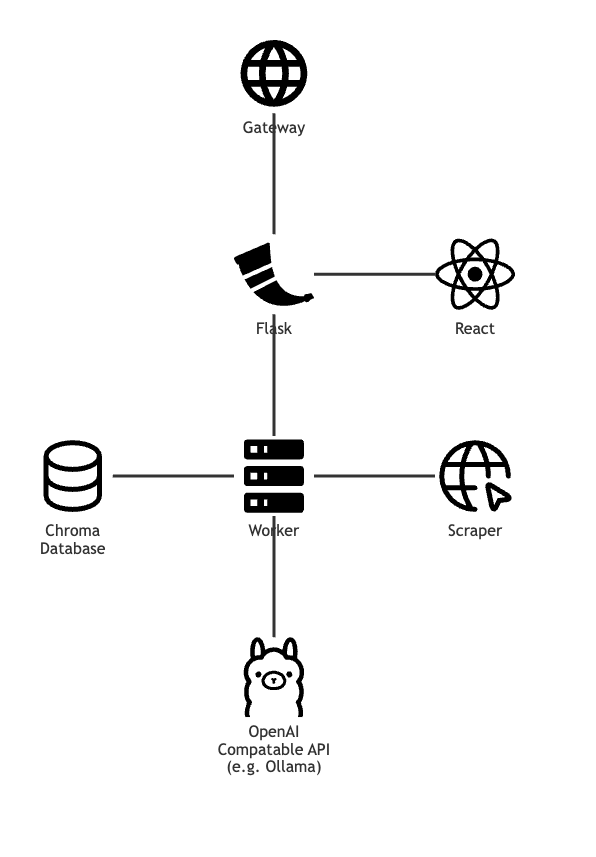
\includegraphics[width=1\linewidth]{final-architecture.png}
    \caption{System Architecture}
    \label{fig:architectureDiagram}
\end{figure}

\subsection{Frontend} % AKA Fronde :fire emoji:
The front-end is built using React, which is a component-based JavaScript library that focuses on creating efficient and modular components \cite{react}. Tailwind CSS provides utility-first styling, which allowed rapid UI development while maintaining consistency across the application \cite{tailwind}.

The front-end communicates with the backend through RESTful API calls, sending article URLs for analysis and receiving structured JSON responses containing the fact-checking results \cite{aws-rest}. React's state management handles the loading states, displaying progress indicators during analysis when available, and rendering the results in an organized, digestible format once they are available. This architecture is designed to handle potentially long-running analyses gracefully, updating the interface progressively as results become available rather than requiring users to wait for the entire process to complete.

\subsection{Backend}
The backend is built on top of a Flask app, a lightweight Python web framework for building APIs \cite{flask}. LLM prompts are routed through a custom LlamaRouter program, which considers all of its possible endpoints (compatible with any OpenAI API compatible endpoint, in practice either Ollama or LlamaCPP), and routes prompts based on server load and token context length to ensure maximum throughput and efficiency without overloading the LLMs themselves \cite{openaiapi, ollama-docs, llamacpp}. Python was chosen as our backend language because the majority of our system's core functionality is best supported in Python, with its vast ecosystem of libraries, particularly for AI and data processing. 
When articles are summarized, they are then passed into three custom agentic LLM frameworks (evaluating accuracy, bias, and completeness), using tool calls to access information on the internet and in our local database. These agents are all run asynchronously, to ensure that they all finish at roughly the same time and are adding to the router queues simultaneously. Each individual fact checking operation is run in its own thread, to allow for concurrency, but all fact checks route through the same LlamaRouter object, causing speed to decrease considerably when running multiple checks at once.

\subsection{Database}
We have used ChromaDB as our vector database for storing and retrieving semantically similar articles \cite{chroma}. Chroma was selected because it allows semantic search using embeddings, which allowed us to find articles on related topics even when they don't share exact terminology. This semantic search capability proved essential given the wide use of language in reporting, as relying solely on keyword matching would have missed relevant articles that use different terminology. Another collection in the same Chroma database is used to store results of past fact checks. Storing it in the same object greatly simplifies accessing the database and making data storage persistent between sessions. We have originally proposed maintaining a standard SQL database to store this alongside user accounts, but with user accounts getting dropped due to time constraints, a standard SQL database will be needed to support user accounts.

\subsection{LLM Selection}
Since our methodology relies heavily on LLMs, present in multiple stages in the analysis pipeline, it is important to choose either a single, well-rounded LLM, or a series of LLMs that are well-suited for each task. These tasks include summarization and extracting key claims, taking points to search for and generating queries for searching in Chroma and across the internet, and final assessment of the articles. Our initial evaluations primarily considered Qwen3\cite{qwen3}, specifically the 8 billion parameter variant, due to its strong performance relative to its size and speed, which allows us to run inference locally with reasonable speed and efficiency, as shown in table \ref{tab:modelBenchmarks}. Additionally, Qwen3 allows structured output and reasoning, allowing the LLM to iterate and take its time on a task before returning machine-readable JSON. This will be crucial in the final assessment portion, as it will allow the LLM to make connections and come to a conclusion of its own, and then output results that can be easily interpreted by the front-end.
\begin{table}[ht]
    \centering
    \caption{Preliminary Model Benchmarks}
    \begin{tabular}{|c|c|c|}
        \hline
        \textbf{\textit{Model}} & \textbf{\textit{Size}} & \textbf{\textit{Time Taken (mean of 10 trials)}} \\ \hline
        Qwen3 8B & 5.2 GB & 25.9 s \\ \hline
        Qwen3 14B & 9.3 GB & 40.3 s \\ \hline
        Qwen3 30B & 18.0 GB & 45.0 s \\ \hline
        Gemma 3 4B & 3.3 GB & 13.8 s \\ \hline
        Gemma 3 12B & 8.1 GB & 41.4 s \\ \hline
        Llama 3 8B & 4.7 GB & 13.7 s \\ \hline
        Llama 3.1 8B & 4.9 GB & 15.2 s \\ \hline
    \end{tabular}
    \label{tab:modelBenchmarks}
\end{table}

\begin{table}[ht]
    \centering
    \caption{Final Model Benchmarks}
    \begin{tabular}{|c|c|c|}
        \hline
        \textbf{\textit{Model}} & \textbf{\textit{Size}} & \textbf{\textit{Time Taken (mean of 30 trials)}} \\ \hline
        Gemma 3 4B & 3.3 GB & 4.268 s \\ \hline
        Gemma 3n e4B & 7.5 GB & 11.689 s \\ \hline
        Gemma 4 e4B & 9.6 GB & 27.249 s \\ \hline
        GLM-4.7-Flash & 19 GB & 150.479 s\\ \hline
        GPT-OSS 20B & 14 GB & 43.61 s \\ \hline
        Llama 3.1 8B & 4.9 GB & 4.768 s \\ \hline
        Nemotron 3 Nano 4B & 2.8 GB & 7.986 s \\ \hline
        Qwen3.5 9B & 6.6 GB & 122.182 s \\ \hline
        Qwen3 8B & 5.2 GB & 11.754 s \\ \hline
    \end{tabular}
    \label{tab:modelBenchmarks2}
\end{table}

In our final version, we elected to use two models: the 4 billion parameter Nemotron-3-Nano for small tasks and article summarization, and GLM-4.7-Flash (an approximately 30 billion parameter mixture of experts model) for our custom agents \cite{nemotron, glm}. In our more recent testing, we found that Nemotron and GLM were both extremely well optimized for our available hardware, and the quality of the output was roughly comparable to the other models we considered. Nemotron was selected due to being extremely lightweight and quick, while GLM was selected for its more robust reasoning and tool use capabilities, while still running reasonably fast on consumer-grade hardware.

\subsection{Prompt Engineering and Assessment} %potentially cite github
For our prompt engineering stage -- creating and refining the LLM prompts for optimal results -- we utilized a custom made script for both testing and evaluating the models and the prompts. The script creates virtual ``agents" with shared specific prompts, and gives them articles to summarize, logging the prompt, model output, and other metrics like processing time for later analysis. (Some of these metrics are shown in tables \ref{tab:modelBenchmarks} and \ref{tab:modelBenchmarks2}.) The script is configured to allow testing of prompts for evaluating the summaries themselves, to use in evaluating the quality of models and prompts beyond pure data. Additionally, since the script can create new agents, back-propagating prompts -- having an LLM rewrite the prompts -- becomes simple, with all past prompts and their results logged. 
In refining our summarizer prompts, we followed a process of writing prompts and getting model output and analyzing that output with a more powerful LLM through the Gemini API, which then gives it a score on the summary's accuracy and completeness. Once we have those scores, we can compare them, as well as the time taken and token cost, between different prompts or different models. Using these comparisons, we can evaluate which model gives us the best results, and find the absolute best prompt we can for that model, making liberal use of back-propagation. We acknowledge that using a high quality LLM to score summary quality is far from objective, but the quality of a summary is subjective and can't be analyzed algorithmically, so using a high powered LLM is the best automated solution we have.
Through the prompt engineering process, we came to the conclusion that accuracy and completeness cannot be assessed separately, and that building an autonomous agentic solution would be the only way to ensure that the models got the information that they needed in the most efficient manner. The previously described prompt engineering script works excellently with agentic prompts as well, and thus the prompt engineering process was almost identical, albeit with somewhat more complex prompts (as the agents need a lot more information to work off of).

\section{Results}
At the end of our 18 days of development, we delivered a largely functional ARGUS web application and server combination that can fact check nearly any article on a distributed system of OpenAI API compatible server endpoints. The initial goal was to have fact checks completed in under 5 minutes, though this was under the assumption that we would have access to a cluster with a NVIDIA A100 Tensor Core GPU, which we did not obtain until after the end of the development period. With our available hardware, consisting of a cluster with 16GB VRAM and two gaming PCs (with 8GB VRAM each), fact checks finish in between 10 and 30 minutes, depending on article complexity. While this does not meet our initial performance goals, we still successfully matched the research time cited for ChatGPT Deep Research -- our most direct competitor -- and our system is fully open source and can run locally.

Going into ARGUS's development, we expected a few primary issues. As with any complex software project involving multiple technologies and AI components, the biggest concern is computing power. Running our own models ensured data security and minimal overhead cost, but required us to actually run the models on our own hardware. Originally this was done through Ollama exclusively, switching between models on the machine running the Flask API. This was functional, but extremely slow due to the constant switching between models on the same device. In later versions, this was addressed by switching the backend to use any OpenAI API compatible endpoint, allowing us to access models hosted on other machines and to run the models with a more efficient framework (in our case, primarily LlamaCPP). The issues with computing power also substantially informed our final model choice, as we went with the models that performed best on our limited hardware rather than those that provided the absolute best output.

The other primary LLM based concern was hallucination, although this was far less of an issue than we expected. With proper prompt engineering and ensuring that the models are able to research any information they want to check, they are generally very good at actually outputting reliable information and citing the sources for their claims. While we did run into some issues regarding this, especially towards the end of the project, it was less of an issue of the LLMs hallucinating new data, and more of the LLMs not adhering to structured output.

Our final concern going in was the reliance on ChromaDB for our article queries. We were not sure of how well Chroma would suit our use case going in, but the ability to query the database using both semantic similarity and with IDs directly suited an agentic application extraordinarily well. Chroma allowed the LLMs to very easily search the database themselves, in addition to allowing easy data retrieval based on a known ID, perfectly suiting everything we needed it for, without any noticeable delays from semantic embedding (which was our primary concern).

In the end, far more of our issues came down to switching LLM prompts from Ollama and the OpenAI endpoints in the backend. This switch provided significant performance increases and allowed us to share the computing load between multiple machines, but caused countless issues with network requests and synchronous/asynchronous Python functions and libraries. By the end of the project it was completely sorted out, but this unforeseen issue became by far the most difficult problem we dealt with in ARGUS's development.

With a longer running development cycle, there would be a large enough amount of data from previous fact checks for intensive analysis. Unfortunately, in our development period, we only successfully analyzed around 40 articles, which is not enough to find any significant patterns in the data. Future investigations would seek to find possible relationships between accuracy/completeness scores and bias scores, to see if a more biased article is necessarily more or less factually correct than a more neutral one. We would also investigate any possible trends between date of reporting and bias scores, or of article topics and their completeness and accuracy scores. All of these would be extremely interesting questions to answer with ARGUS analytics, but any analysis on our current dataset would be practically useless due to the small sample size, and providing any substantial statistical analysis would only be misleading. 

\section{Conclusion}
In the age of misinformation and AI generated content online, ARGUS delivers a solution for autonomously fact checking news articles at a level that can be run locally on any reasonably powerful computer, and can be seamlessly scaled up with any number of endpoints. Quantifying the truth of an article is nearly impossible, but ARGUS reliably analyzes the key points of the article and autonomously researches the factual accuracy of the points, the reporting completeness of the article, and assesses the article's bias, all while citing its sources to ensure users can check its work. It is not a 100\% reliable checker, but it successfully automates the process and gives users the tools to verify its accuracy. In the future, the system could be made more efficient using some form of dynamic context clearing to reduce loads on the LLMs themselves, and further tweaks could be made to prompts and formatting to ensure reliable output more frequently. 

% \begin{thebibliography}{00}
% TODO: get bibtex for bibliography
% currently looking for artifacts.bib, but we just need to rename it.
\bstctlcite{IEEEexample:BSTcontrol}
\bibliographystyle{IEEEtran}
\bibliography{artifacts}

%https://grokaimodel.com/misinformation/

% \end{thebibliography}
\end{document}
